%%%%%%%%%%%%%%%%%%%%%%%%%%%%%%%%%%%%%%%%%
% University Assignment Title Page 
% LaTeX Template
% Version 1.0 (27/12/12)
%
% This template has been downloaded from:
% http://www.LaTeXTemplates.com
%
% Original author:
% WikiBooks (http://en.wikibooks.org/wiki/LaTeX/Title_Creation)
%
% License:
% CC BY-NC-SA 3.0 (http://creativecommons.org/licenses/by-nc-sa/3.0/)
% 
% Instructions for using this template:
% This title page is capable of being compiled as is. This is not useful for 
% including it in another document. To do this, you have two options: 
%
% 1) Copy/paste everything between \begin{document} and \end{document} 
% starting at \begin{titlepage} and paste this into another LaTeX file where you 
% want your title page.
% OR
% 2) Remove everything outside the \begin{titlepage} and \end{titlepage} and 
% move this file to the same directory as the LaTeX file you wish to add it to. 
% Then add \input{./title_page_1.tex} to your LaTeX file where you want your
% title page.
%
%%%%%%%%%%%%%%%%%%%%%%%%%%%%%%%%%%%%%%%%%

%----------------------------------------------------------------------------------------
%	PACKAGES AND OTHER DOCUMENT CONFIGURATIONS
%----------------------------------------------------------------------------------------

\documentclass[12pt]{article}
\usepackage[utf8]{inputenc}
\usepackage[russian]{babel}
\usepackage{amsmath,amsfonts,amsthm} % Math packages
\usepackage{mathtools}
\usepackage{graphicx}
\usepackage{booktabs}
\usepackage[margin=1.15in]{geometry}
\DeclareGraphicsExtensions{.pdf,.png,.jpg}

\usepackage{lipsum} % Used for inserting dummy 'Lorem ipsum' text into the template

\usepackage{sectsty} % Allows customizing section commands
\allsectionsfont{\centering \normalfont\scshape} % Make all sections centered, the default font and small caps

\usepackage{fancyhdr} % Custom headers and footers
\pagestyle{fancyplain} % Makes all pages in the document conform to the custom headers and footers
\fancyhead{} % No page header - if you want one, create it in the same way as the footers below
\fancyfoot[L]{} % Empty left footer
\fancyfoot[C]{} % Empty center footer
\fancyfoot[R]{\thepage} % Page numbering for right footer
\renewcommand{\headrulewidth}{0pt} % Remove header underlines
\renewcommand{\footrulewidth}{0pt} % Remove footer underlines
\setlength{\headheight}{13.6pt} % Customize the height of the header

\numberwithin{equation}{section} % Number equations within sections (i.e. 1.1, 1.2, 2.1, 2.2 instead of 1, 2, 3, 4)
\numberwithin{figure}{section} % Number figures within sections (i.e. 1.1, 1.2, 2.1, 2.2 instead of 1, 2, 3, 4)
\numberwithin{table}{section} % Number tables within sections (i.e. 1.1, 1.2, 2.1, 2.2 instead of 1, 2, 3, 4)

\setlength\parindent{0pt} % Removes all indentation from paragraphs - comment this line for an assignment with lots of text

\begin{document}

\begin{titlepage}

\newcommand{\HRule}{\rule{\linewidth}{0.5mm}} % Defines a new command for the horizontal lines, change thickness here

\center % Center everything on the page
 
%----------------------------------------------------------------------------------------
%	HEADING SECTIONS
%----------------------------------------------------------------------------------------

\textsc{\Large київський національний університет імені тараса шевченка}\\[1.5cm] % Name of your university/college
\textsc{\large факультет комп'ютерних наук та кібернетики}\\[0.5cm] % Major heading such as course name
\textsc{\large фафедра прикладної математики}\\[0.5cm] % Minor heading such as course title

%----------------------------------------------------------------------------------------
%	TITLE SECTION
%----------------------------------------------------------------------------------------

\HRule \\[0.4cm]
{ \Large \bfseries Лабораторна робота №1 з курсу “Чисельні методи математичної фізики”:}\\[0.4cm] % Title of your document
{ \Large \bfseries “Розв'язання граничної задачі методом Бубнова-Галеркіна та методом найменших квадратів” }
\HRule \\[1.5cm]
 
%----------------------------------------------------------------------------------------
%	AUTHOR SECTION
%----------------------------------------------------------------------------------------

\begin{minipage}{0.4\textwidth}
\begin{flushleft} \large
\emph{Студент 4-го курсу}\\
\emph{групи ОМ}\\
Чан Ха Ву % Your name
\end{flushleft}
\end{minipage}
~
\begin{minipage}{0.4\textwidth}
\begin{flushright} \large
\emph{Викладач:} \\
\emph{к.ф.-м.н., доцент} \\
Риженко \textsc{А. І.} % Supervisor's Name
\end{flushright}
\end{minipage}\\[4cm]

% If you don't want a supervisor, uncomment the two lines below and remove the section above
%\Large \emph{Author:}\\
%John \textsc{Smith}\\[3cm] % Your name

%----------------------------------------------------------------------------------------
%	DATE SECTION
%----------------------------------------------------------------------------------------

{\large Київ, 23 грудня 2016}\\[3cm] % Date, change the \today to a set date if you want to be precise

%----------------------------------------------------------------------------------------
%	LOGO SECTION
%----------------------------------------------------------------------------------------

%\includegraphics{Logo}\\[1cm] % Include a department/university logo - this will require the graphicx package
 
%----------------------------------------------------------------------------------------

\vfill % Fill the rest of the page with whitespace
\end{titlepage}

%----------------------------------------------------------------------------------------
%	ПОСТАНОВКА ЗАДАЧИ
%----------------------------------------------------------------------------------------
\section{Постановка задачі}

Методом Бубнова-Галеркіна та методом найменших квадратів знайти розв’язок граничної задачі для звичайного диференціального рівняння другого порядку

\begin{align} \label{problem}  
\begin{split}
-\frac{d}{dx} \left( k(x)\frac{du}{dx} \right) + p(x)\frac{du}{dx} + q(x)u = f(x), \quad a < x < b
\end{split}					
\end{align}

з наступними умовами

\begin{align} \label{conditions}  
\begin{split}
-k(x)\frac{d}{dx}u(x) + \alpha_1 u(x) = \mu_1(x), \quad x = a \\
k(x)\frac{d}{dx}u(x) + \alpha_2 u(x) = \mu_2(x), \quad x = b
\end{split}					
\end{align}

де $\alpha_1 > 0, \alpha_2 > 0$. Треба побудувати графік для наближеного розв'язку та апроксимизації. Порівняти з точним (аналітичним) розв'язком.



%----------------------------------------------------------------------------------------
%	ТОЧНОЕ РЕШЕНИЕ
%----------------------------------------------------------------------------------------
\section{Точний розв'язок}

При наступному вигляді функції $k$, $p$ та $q$:

\begin{equation} \label{analytical_solution}  
\begin{split}
k(x) = k_1 cos(k_2 x) + k_3, \quad k(x) > 0 \\
p(x) = p_1 sin(p_2 x) + p_3, \quad p(x) > 0 \\
q(x) = q_1 cos(q_2 x) + q_3, \quad q(x) > 0 \\
\end{split}					
\end{equation}

Нехай функція $f$ набуває наступний вигляд:

\begin{equation}
\begin{multlined} \label{analytical_solution}  
f(x) = k_1 k_2 m_1 m_2 \cos(m_2 x) \sin(k_2 x) + \\ + m_1 m_2^2 \left(k_1 \cos(k_2 x) + k_3 \right)\sin(m_2 x) + p_1 m_1 m_2 \cos(m_2 x) \sin(p_2 x) + \\ +
p_3 m_1 m_2 \cos(m_2 x)
\end{multlined}
\end{equation}

та нехай коефіцієнти $\mu_1$, $\mu_2$ дорівнюють

\begin{align}
\begin{split}
\mu_1 = k(x)\frac{d}{dx}\left(m_1 sin(m_2 x) + m_3 cos(m_4 x) + m_5 \right)(a) - \\ - \alpha_1 \left(m_1 sin(m_2 a) + m_3 cos(m_4 a) + m_5 \right) \\
\mu_2 = - k(x)\frac{d}{dx}\left(m_1 sin(m_2 x) + m_3 cos(m_4 x) + m_5 \right)(b) - \\ - \alpha_2 \left(m_1 sin(m_2 b) + m_3 cos(m_4 b) + m_5 \right)
\end{split}
\end{align}

У такому випадку, точний (аналітичний) розв'язок задачі \ref{problem} набуває наступний вигляд:

\begin{equation} \label{analytical_solution}  
\begin{split}
u(x) = m_1 sin(m_2 x) + m_3 cos(m_4 x) + m_5
\end{split}					
\end{equation}



%----------------------------------------------------------------------------------------
%	ТЕОРЕТИЧЕСКИЕ ВЕДОМОСТИ
%----------------------------------------------------------------------------------------

\section{Теоретичні відомості}

Нехай задано рівняння

\begin{equation}  \label{uravnenie}
\begin{split}
Lu = f
\end{split}					
\end{equation}

де $L: H \rightarrow H$ -- лінійний диференціальний оператор на певному гільбертовому просторі $H$, $f \in H$, $u$ -- невідома функція.
При чому додається однородні граничні крайові умови:

\begin{equation} \label{kraevaya_zad}
\begin{split}
\alpha_1 u(a) - \alpha_2 u'(a) = 0, \quad |\alpha_1| + |\alpha_2| \neq 0, \quad \alpha_1 \alpha_2 \geq 0 \\
\beta_1 u(b) - \beta_2 u'(b) = 0, \quad |\beta_1| + |\beta_2| \neq 0, \quad \beta_1 \beta_2 \geq 0 \\
\end{split}					
\end{equation}


При використанні будь-якого з проекційних методів обирається лінійно-незалежна система функції $\phi_1(x), \phi_2(x), \dots \phi_n(x)$, яку будемо називати координатами, і приблизьний розв'язок щукається у вигляді лінійної комбінації цих функцій

\begin{equation} \label{priblizitelno}
\begin{split}
y^{(n)}(x) = \sum_{i=1}^n {c_i \phi_i (x)}.
\end{split}					
\end{equation}

Коефіцієнти розкладу $c_i$ є розв'язком лінійної системи

\begin{equation} 
\begin{split}
\sum_{j=1}^N {a_{ij} c_j = f_i}, \quad i = 1, 2, \dots n
\end{split}					
\end{equation}

Спосіб побудови матриці $G = \{ a_{ij} \}_{i,j = 1}^{n} $ та вектора $F = (f_1, f_2 \dots, f_n)'$ залежить від обраного проекційного методу.

\subsection{Метод найменших квадратів}

Очевидно що розв'язок $y^*$ крайової задачі \ref{kraevaya_zad} для рівняння \ref{uravnenie} також мінімізує функціонал 

\begin{equation} 
\begin{split}
\omega(u) = \| Lu - f \|^2 = (Lu - f, Lu - f)
\end{split}					
\end{equation}

заданому на множині $D(L)$. В методі найменших квадратів, пощук коефіцієнтів $c_i$ у приблизьному розв'язку \ref{priblizitelno} зводиться до розв'язку матричного рівняння:

\begin{equation} 
\begin{split}
\sum_{i=j}^{n} c_j (L\phi_i, L\phi_j) = (f, L\phi_i), \quad i = 1, 2, \dots n
\end{split}					
\end{equation}

\subsection{Метод Бубнова-Галеркіна}

В методі найменших квадратів, коефіцієнти $c_i$ у приблизьному розв'язку \ref{priblizitelno} щукається за допомогою системи:

\begin{equation} 
\begin{split}
\sum_{i=j}^{n} c_j (\phi_i, L\phi_j) = (f, \phi_i), \quad i = 1, 2, \dots n
\end{split}					
\end{equation}

Цю систему можна трактувати як умова ортогональності в $L_2$ нев'язки $Lu_n - f$ всім функціям координатної системи.

%----------------------------------------------------------------------------------------
%	ПРАКТИЧНА ЧАСТИНА
%----------------------------------------------------------------------------------------

\section{Практична частина}

%Обчислимо спочатку $f$ і $\mu_1, \mu_2$, виходячи з того, що ми знаємо, що %функція $u$ (розв'язок) виглядає як $u(x) = m_1 x^{m_2} + m_3 x^{m_4} + m_5$. Тому ми просто можемо підставити розв'язок u у крайові умови \ref{conditions}.

\bigskip

Маємо неоднорідні краєві умови. Тому розв'язок будемо шукати у вигляді $u = v + \psi$, де $\psi = cx + d$. Функція $\psi$ буде задовольняти неоднорідним крайовим умовам, тому функція $v$ вже буде задовольнати однорідним крайовим умовам. Для знаходження коефіцієнтів $c,d$ підставимо функцію $\psi$ в крайові умови і розв'яжемо систему з двох рівнянь.

	\begin{equation*}
	\begin{split}
	-k(a)\psi'(a) + \alpha_1 \psi(a) = \mu_1 \\ 
	k(b)\psi'(b) + \alpha_2 \psi(b) = \mu_2
	\end{split}
	\end{equation*}

Звідси отримуємо:

	\begin{equation}
	\begin{split}
c = \frac{-(\alpha_2 \mu_1 - \alpha_1 \mu_2)}{\alpha_2\alpha_1(b-a) + \alpha_2 k(a) + alpha_1 k(b)} \\
d = \frac{(-a \alpha_1 \mu_2 + b \alpha_2 \mu_1 + k(a) \mu_2 + \mu_1 k(b)}{\alpha_2\alpha_1(b-a) + \alpha_2 k(a) + alpha_1 k(b)}
	\end{split}
	\end{equation}
	
Після цього перераховуємо функцію  $f$ для того, щоб знайти вигляд рівняння для $v$:
	
	\begin{equation}
	\begin{split}
	f_1(x) = f(x) - \left( -(k\psi')' + p(x)\psi' + q(x)\psi \right)
	\end{split}
	\end{equation}
	
Задамо систему функцій $\phi$ для методу колокації у вигляді 

	\begin{align}
	\phi_i(x) = 
	\begin{cases}
	(x - a)^2(x - A), & i = 1 \\ 
	(x - b)^2(x - B), & i = 2 \\
	(x - a)^{i -1}(x - b)^2 & i = 3, \dots n
	\end{cases}
	\end{align}

Для знаходження невідомих коефіцієнтів $A$ та $B$ підставимо ці функції у вже однорідні крайові умови. Треба розв'язати таку систему рівнянь: 
	
	\begin{equation}
	\begin{split}
	-k(a)\phi_2'(a) + \alpha_1 \phi_2(a) = \mu_1 \\ 
	k(b)\phi_1'(b) + \alpha_2 \phi_1(b) = \mu_2
	\end{split}
	\end{equation}
	
Звідси

	\begin{equation}
	\begin{split}
	A = \frac{-k(b)(a-b)(a-3b) - \alpha_2(b-a)^2b}{2k(b)(a-b) - \alpha_2(b-a)^2} \\
	B = \frac{k(a)(b-a)(b-3a) - \alpha_1(a-b)^2a}{-2k(a)(b-a)2 - \alpha_1(a-b)^2}
	\end{split}
	\end{equation}

Така система функції задовольняє однорідним крайовим умовам \ref{conditions}, а значить, чисельний розв'язок для $v$ у вигляді \ref{priblizitelno} теж буде задовольняти цим умовам.



%----------------------------------------------------------------------------------------
%	РЕЗУЛЬТАТ РОБОТИ
%----------------------------------------------------------------------------------------

\section{Результат роботи програми}

Надалі колір для функцій: зелений -- точний розв'язок, маджента(пурпурний) - чисельний розв'язок.

\bigskip

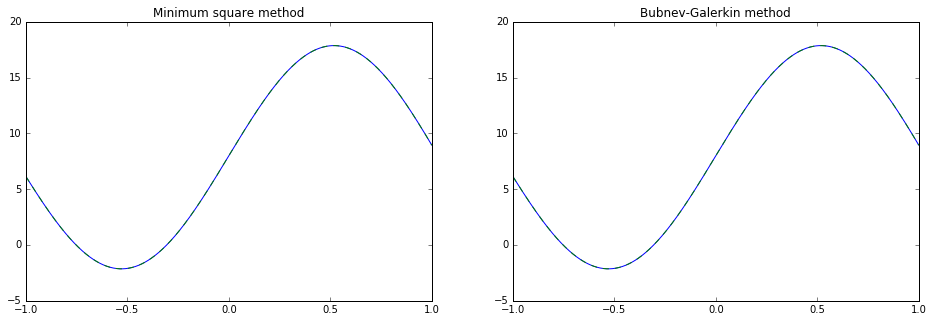
\includegraphics[width=1\linewidth]{res.png}

\begin{center}
	%                 n   a   b   m1  m2  m3  m4  m5  k1  k2  k3  p1  p2  p3  q1  q2  q3  a1  a2
    \begin{tabular}{| l | l | l | l | l | l | l | l | l | l | l | l | l | l | l | l | l |}
	\hline
	n & a & b & $m_1$ & $m_2$ & $m_3$ & $m_4$ & $m_5$ & $k_1$ & $k_2$ & $k_3$ & $p_1$ & $p_2$ & $p_3$ & $q_1$ & $q_2$ & $q_3$ \\ \hline
	10 & -1 & 1 & 10 & 3 & 1 & 1 & 7 & 1 & 2 & 1 & 4 & 1 & 3 & 1 & 2 & 1 \\ \hline


    \end{tabular}
\end{center}

\end{document}